\documentclass[../main/main.tex]{subfiles}

\newdate{date}{30}{10}{2020}


\begin{document}

\marginpar{ \textbf{Laboratory 10.} \\  \displaydate{date}. \\ Compiled:  \today.}

Abbiamo continuato il cablaggio, in particolare il tracciamento dei fili nella camera. In particolare, il circuito finale e il cablaggio dei fili si capisce visualizzando Fig. \ref{fig:10_4} e Fig. \ref{fig:10_5}.

\begin{figure}[h!]
\centering
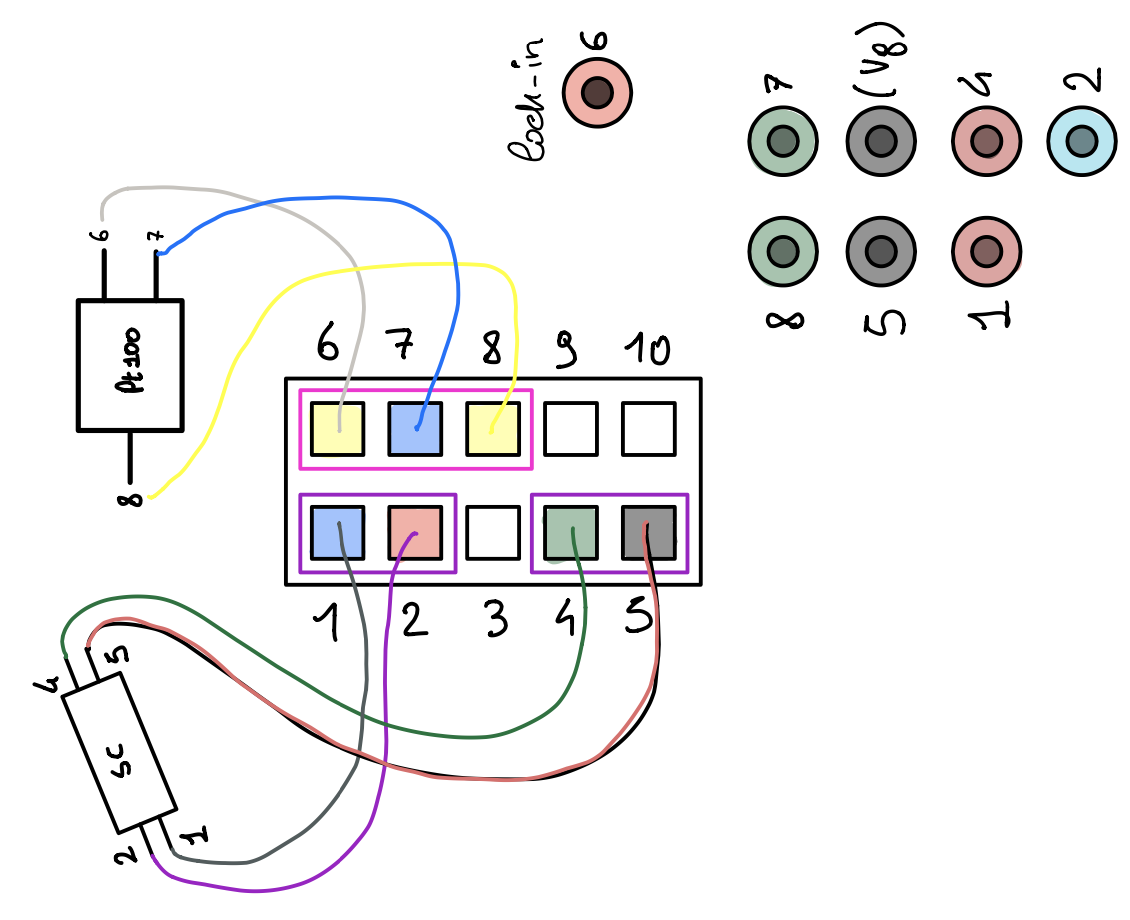
\includegraphics[width=0.8\textwidth]{../lessons/image/10/4.png}
\caption{\label{fig:10_4} Cablaggio dei fili.}
\end{figure}

\begin{figure}[h!]
\centering
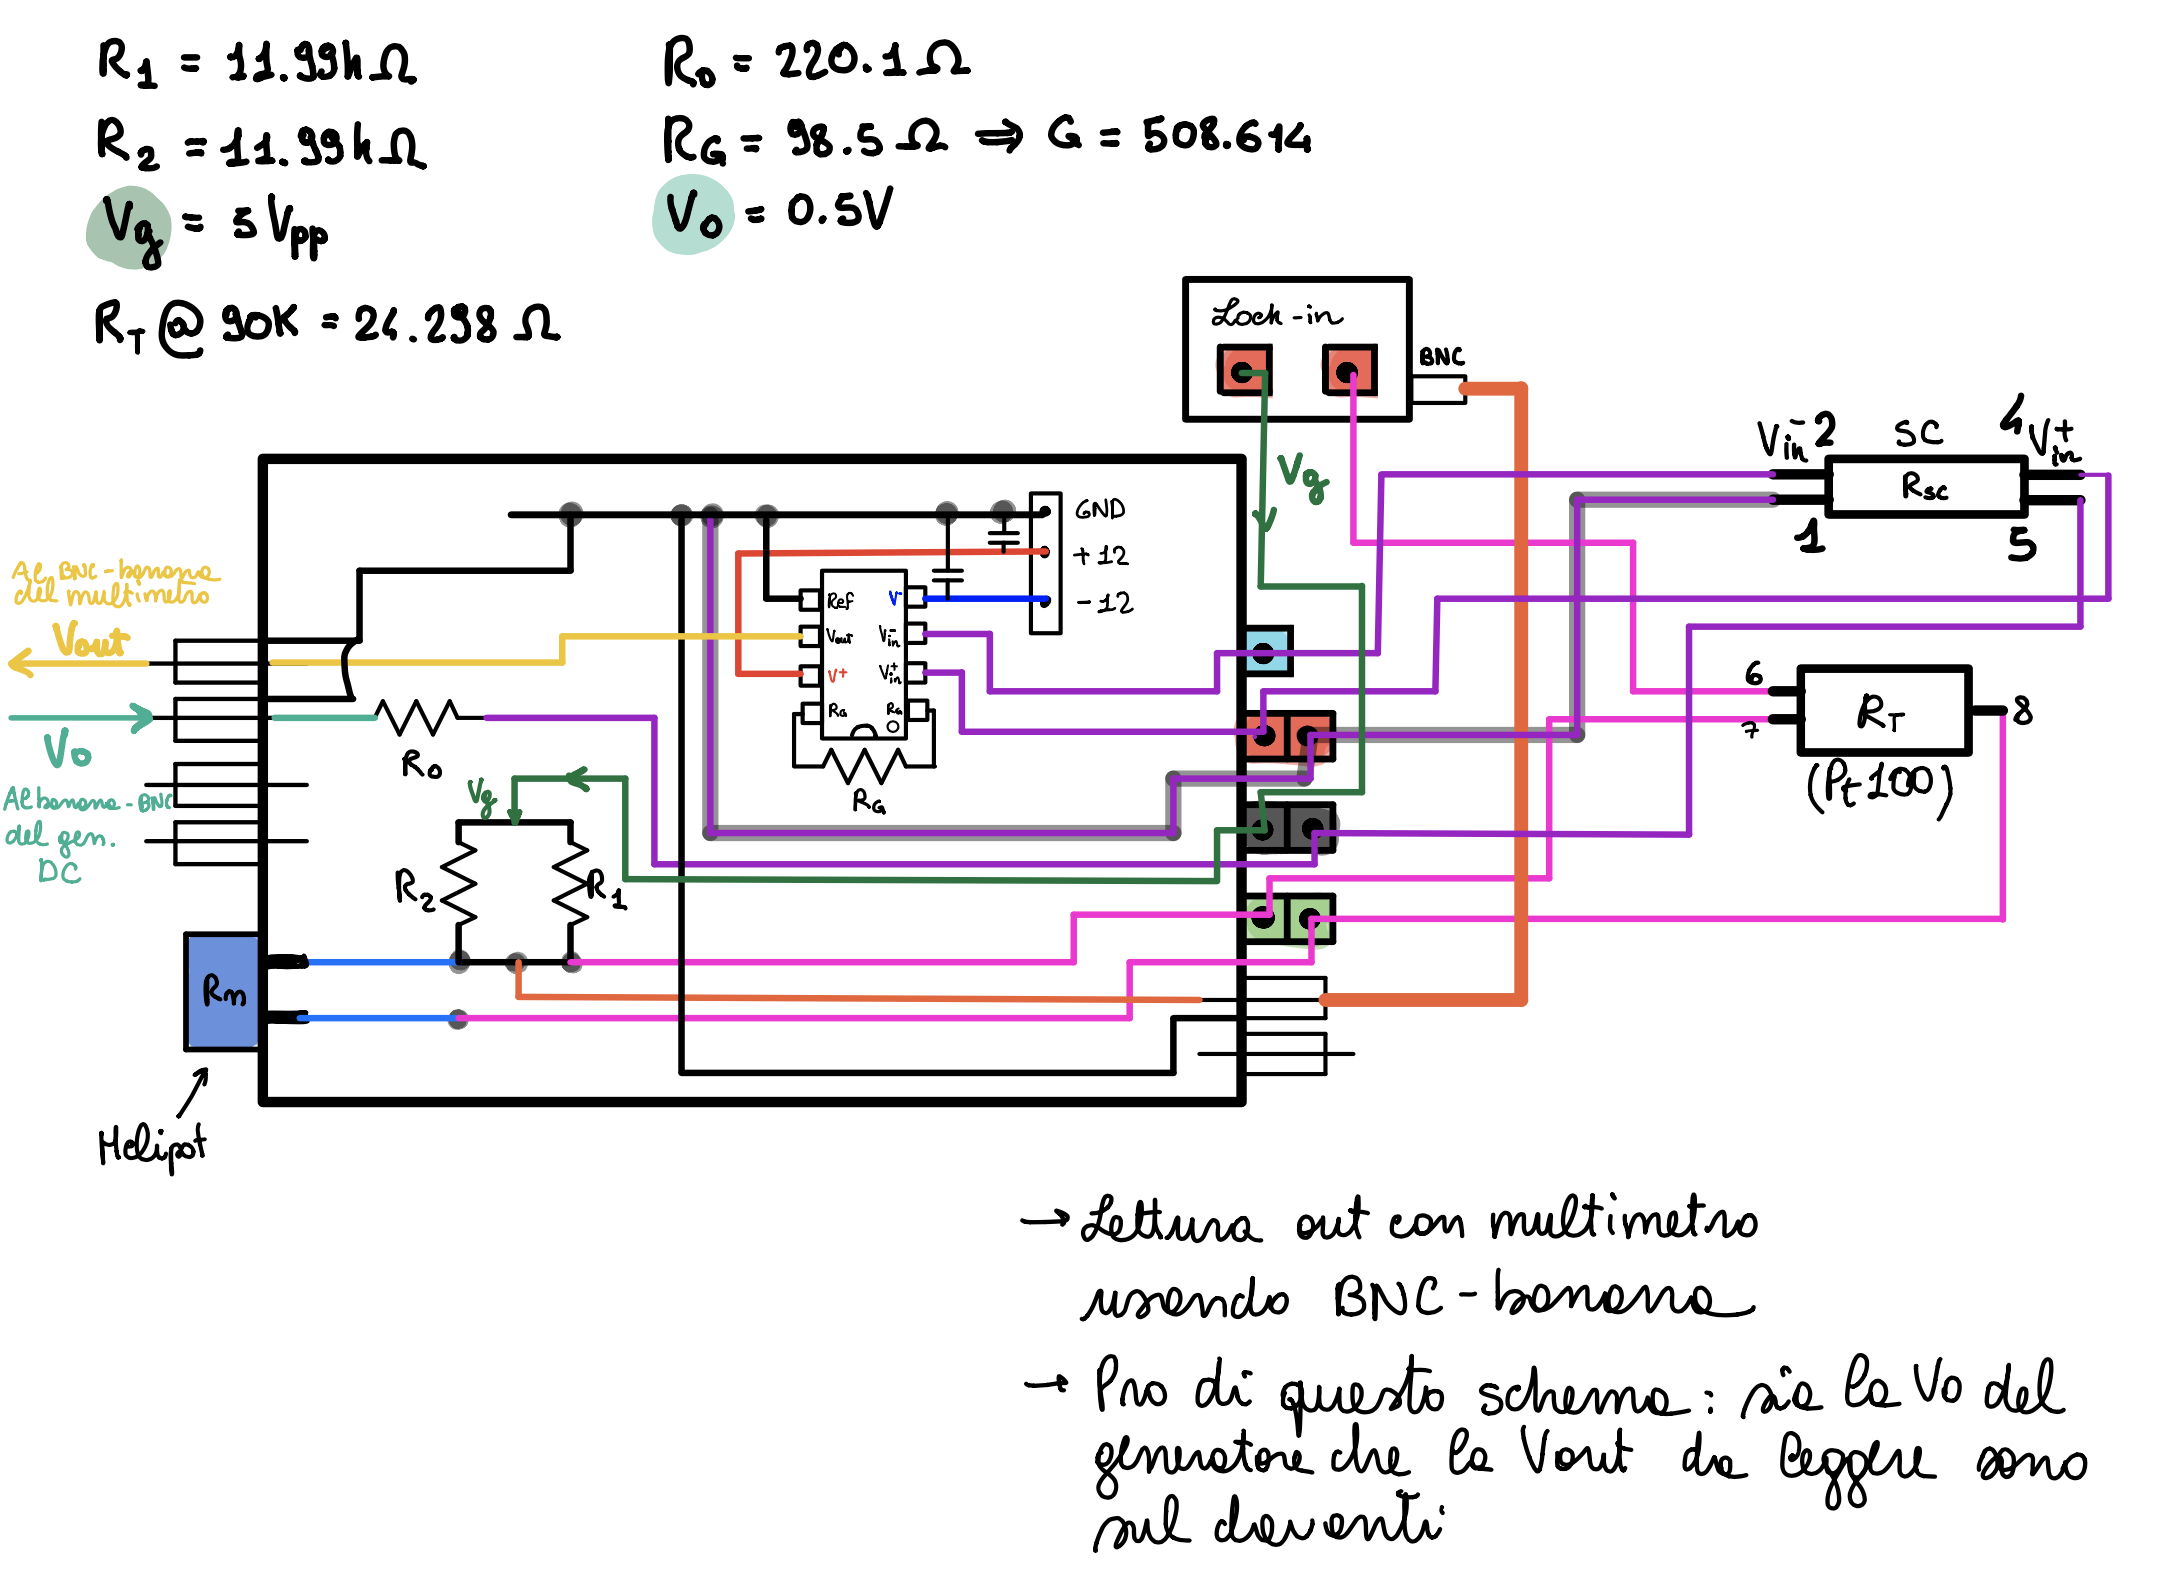
\includegraphics[width=1\textwidth]{../lessons/image/10/5.png}
\caption{\label{fig:10_5} Circuito finale + cablaggio fili.}
\end{figure}

Il pezzo è montato nella camera con in Fig. \ref{fig:10_3}.

\begin{figure}[h!]
\centering
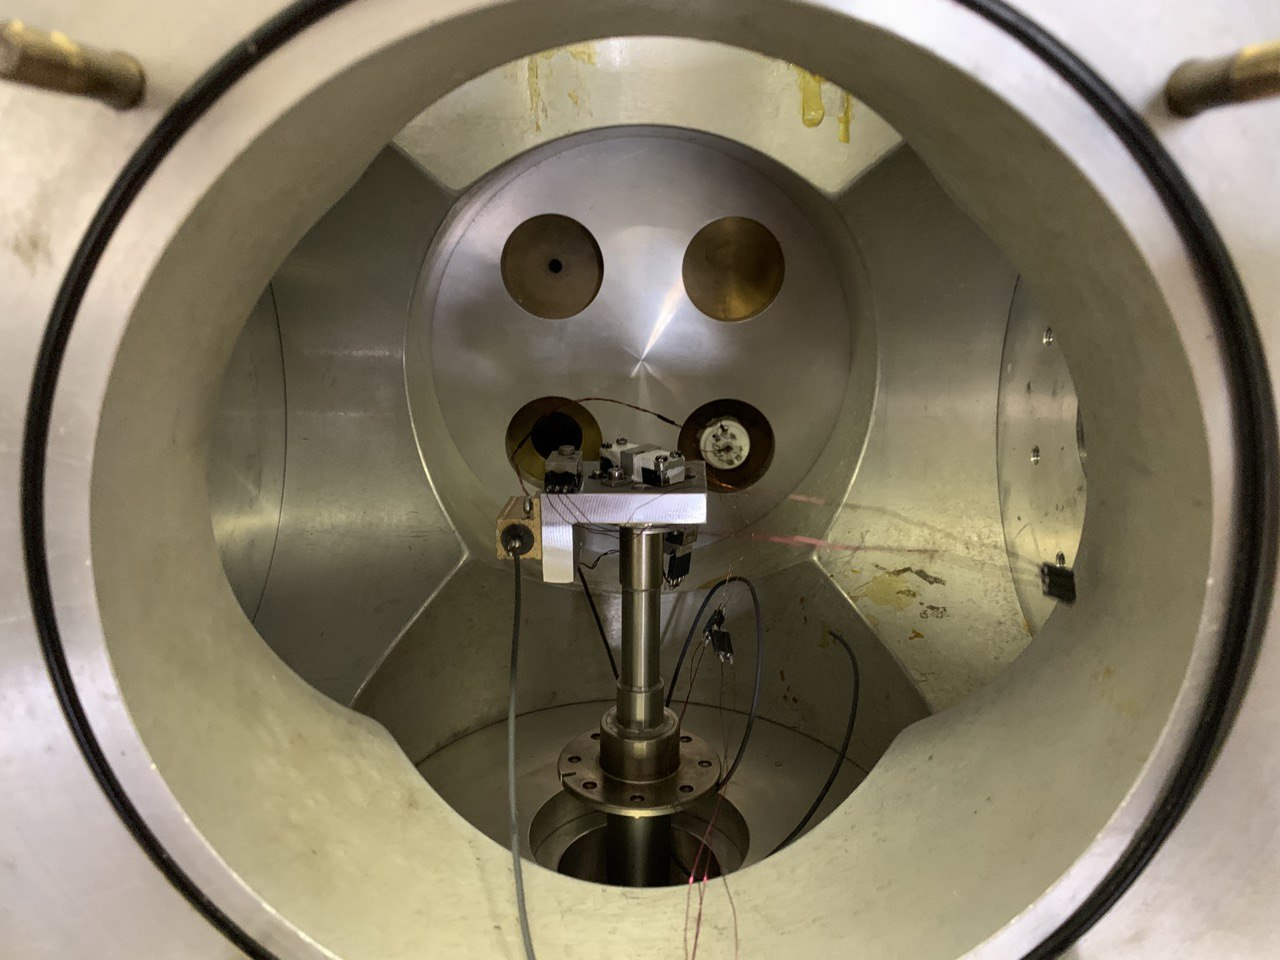
\includegraphics[width=0.8\textwidth]{../lessons/image/10/3.jpg}
\caption{\label{fig:10_3} Come il campione è montato nella camera.}
\end{figure}


Abbiamo poi finito di saldare tutto e preparare il setup sperimentale. Dovrebbe essere tutto pronto a meno di problemi.
Il circuito finale montato è come in Fig. \ref{fig:10_1}.

\begin{figure}[h!]
\centering
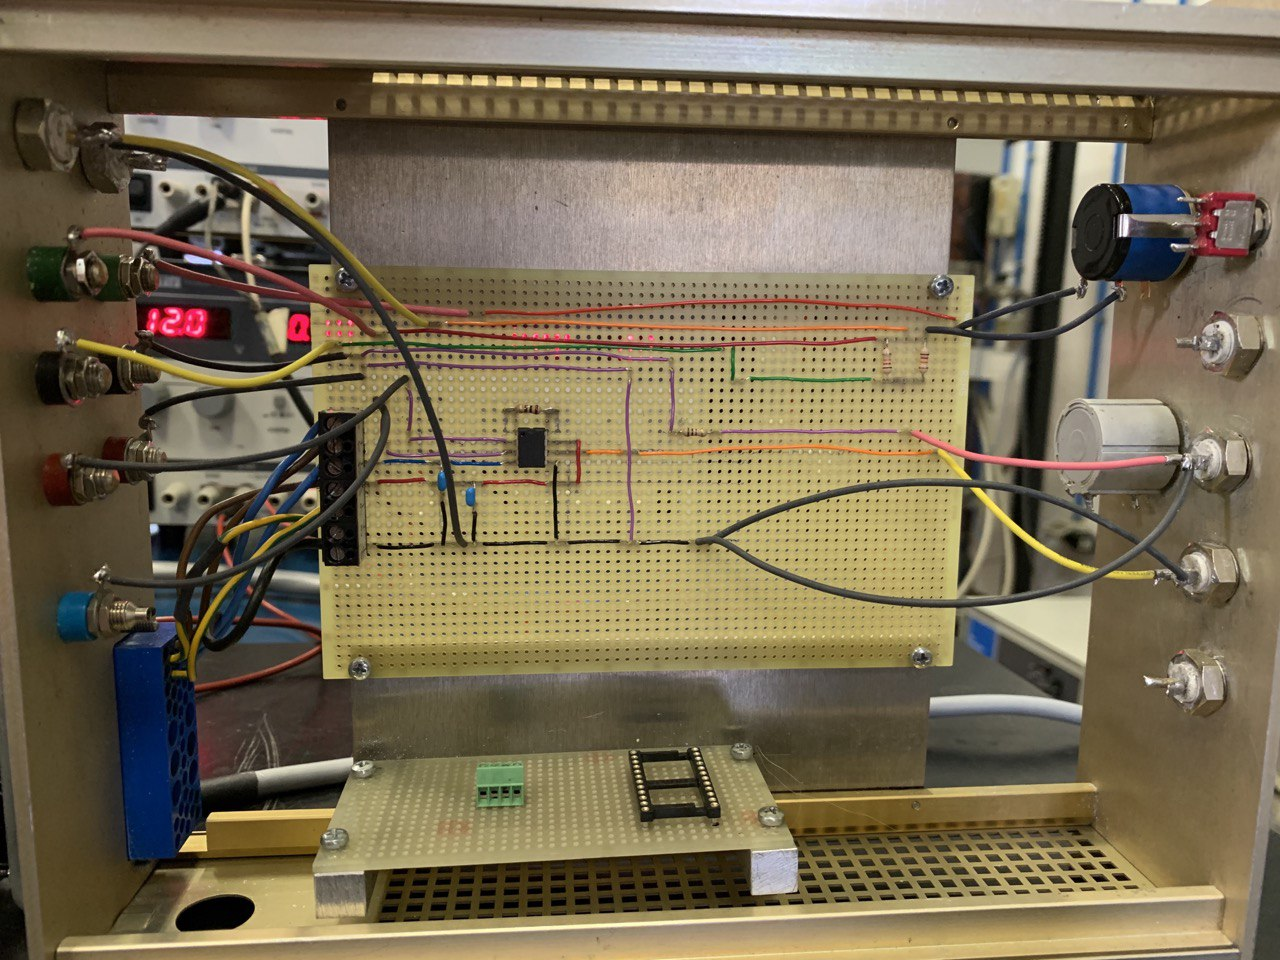
\includegraphics[width=0.8\textwidth]{../lessons/image/10/1.jpg}
\caption{\label{fig:10_1} Circuito finale a meno di errori nella saldatura.}
\end{figure}

Il montaggio del modulo NIM è come in Fig. \ref{fig:10_2}.

\begin{figure}[h!]
\centering
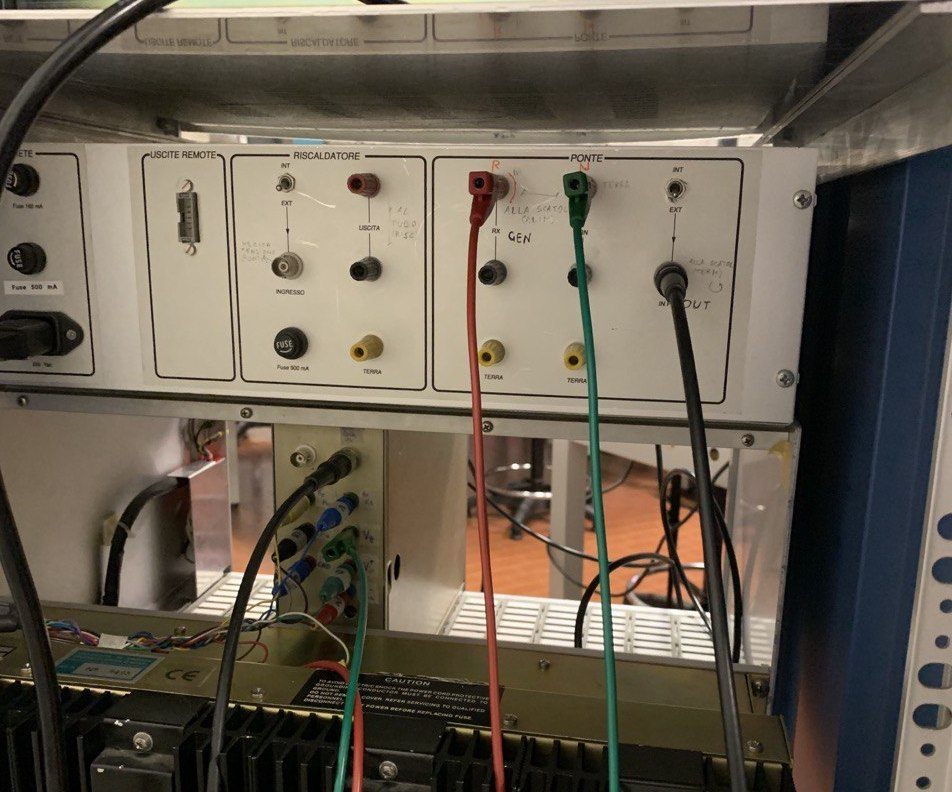
\includegraphics[width=0.8\textwidth]{../lessons/image/10/2.jpg}
\caption{\label{fig:10_2} Modulo NIM montato (immagine del retro con il collegamento del lock-in).}
\end{figure}



\clearpage

\section{Breve lezione su Arduino}
\marginpar{ \textbf{Laboratory 11.} \\  \displaydate{date}. \\ Compiled:  \today.}

Andremo ad utilizzare ingressi con frequenza di campionamento di 10 kHz. Si collega al computer con cavo USB, ma il protocollo di comunicazione con la porta è seriale. La potenza della scheda dta in questo cip di comunicazione.
Il cuore della scheda è il microcontrollore. Abbiamo 13 pin digitali, che possono essere programmati sia come ingressi che uscite digitali. Quindi stiamo lavorando a 5 V. La risoluzione è di 5 mV (abbiamo 10 bit). La porta USB oltre che la comunicazione permette di alimentare la scheda.

Non serve definire gli ingressi analogici, se invece utilizzassi quelli digitali devo dire come viene settato il pin (se ingresso o uscita).
La massima acquisizione che si può fare con l'analogico è di 10 kHz.

Nel nostro caso l'arduino utilizza 5 V che è esattamente la tensione erogata dal pc. Possiamo anche alimentare l'arduino con una tensione esterna che va da 7 a 12 V.

\begin{remark}
IMPORTANTE: il segnale che diamo in pasto all'arduino deve essere compreso tra 0 e 5 V. In caso contrario si rischia di bruciare la scheda.
\end{remark}


\subsection{LabView}
La prima parte del programma dice al pc con che tipo di seriale ci stiamo connettendo. Poi abbiamo dei caratteri che ci dicono l'ingresso che stiamo leggendo. Poi c'è un'icona di selezione etc etc.






\end{document}
